\addchap{Résumé}

Dans cette thèse, nous étudions le type d'homotopie des espaces de configuration de variétés en utilisant des idées venant de la théorie des opérades.
Ces espaces de configuration consistent en des collections de points deux à deux distincts dans une variété donnée.
Nous répondons aux problèmes de l'invariance homotopique et de la définition de modèles rationnels de ces espaces.
Nous adaptons et généralisons des constructions de Kontsevich, qui donnent la formalité des espaces de configuration (compactifiés) des espaces euclidiens en tant qu'opérade~\cite{Kontsevich1999}.

La notion d'opérade fut initialement introduite dans le but d'étudier les espaces de lacets itérés en théorie de l'homotopie~\cite{May1972,BoardmanVogt1973}.
La théorie a connu une renaissance considérable au milieu des années 90 quand, inspirés par un article de Kontsevich~\cite{Kontsevich1993a}, Ginzburg et Kapranov~\cite{GinzburgKapranov1994} ont démontré dans des travaux fondateurs que certains phénomènes de dualité en algèbre pouvaient s'interpréter en termes d'opérades.
Depuis, de nombreuses nouvelles applications des opérades ont été découvertes dans plusieurs domaines des mathématiques.

\addsec{Introduction}

\subsection*{Opérades}

Une opérade est un objet qui gouverne une catégorie d'algèbres.
L'idée centrale de la théorie peut s'expliquer par analogie avec la théorie des représentations de groupes.
Dans cette analogie, l'opérade correspond au groupe, et les algèbres sur l'opérade correspondent aux représentations du groupe.

Si un groupe est défini par une présentation par générateurs et relations, alors la catégorie de ses représentations peut se définir en termes des actions des générateurs sujettes aux relations.
Dans notre analogie, une catégorie d'algèbres est définie par des opérations génératrices et des relations.
Par exemple, la structure d'une algèbre associative se définit par une opération génératrice, le produit, et une relation, l'associativité.
La structure d'une algèbre commutative se définit de façon similaire, avec la condition supplémentaire de symétrie du produit.
Les algèbres de Lie sont définies par un crochet antisymétrique et la relation de Jacobi, etc.
Nous pouvons interpréter chacune de ces définitions comme la définition d'une opérade par générateurs et relations qui gouvernerait la catégorie d'algèbres en question.

Tout comme nous étudions les groupes, il est intéressant d'étudier l'opérade elle-même, indépendamment de toute présentation par générateurs et relations.
Cette nouvelle perspective nous permet de parler de morphismes, de sous-opérades, de quotients, d'extensions, etc., et de traduire des informations sur une opérade en des informations sur la catégorie des algèbres sur cette opérade.

Expliquons plus précisément ce qu'est une opérade.

\begin{wrapfigure}{l}{0.3\textwidth}
  \centering
  \vspace{-5mm}
  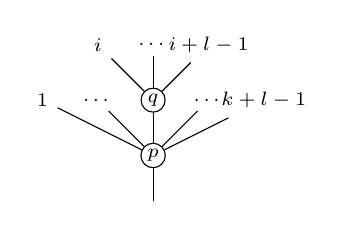
\begin{tikzpicture}[font=\scriptsize, grow'=up, level 1/.style={sibling distance=2em, level distance=2em}]
    \node{}
    child {
      node[draw, circle, inner sep = 1 pt] {$p$}
      child {node {$1$}}
      child {node {\dots}}
      child {
        node[draw, circle, inner sep = 1pt] {$q$}
        child {node {$i$}}
        child {node {\dots}}
        child {node {$i+l-1$}}
      }
      child {node {\dots}}
      child {node{$k+l-1$}}
    }
    ;
  \end{tikzpicture}
  \vspace{-5mm}
\end{wrapfigure}


Les structures algébriques associées aux opérades sont celles qui peuvent être décrites en termes d'opérations avec un nombre fini d'entrées et exactement une sortie.
Une opérade\footnote{Pour nous, une «opérade» sans autre qualificatif est une opérade symétrique à une couleur. Il existe d'autres variantes : opérades non symétriques, opérades cycliques, opérades colorées, etc.} $\PP$ est une collection $\PP = \{ \PP(k) \}_{k \geq 0}$ «d'opérations» abstraites.
On peut voir un élément de $\PP(k)$ comme une opération à $k$ entrées et une sortie.
Le groupe symétrique $\Sigma_{k}$ agit sur $\PP(k)$, ce qui correspond à la permutation des entrées d'une opération.
Il faut également se donner des opérations d'insertion
\[ \circ_{i} : \PP(k) \otimes \PP(l) \to \PP(k+l-1), \quad 1 \leq i \leq k, \]
qui modélisent la composition des opérations (tout comme la multiplication dans un groupe $G$ correspond à la composition des actions sur les représentations).
Enfin, une identité $\id \in \PP(1)$ est un élément neutre pour la composition.

Pour illustrer cette définition, considérons l'exemple prototypique, l'\emph{opérade des endomorphismes}.
Étant donné un objet $X$ dans une catégorie monoïdale symétrique, l'opérade des endomorphismes $\End_{X}$ est définie par $\End_{X}(n) \coloneqq \Hom(X^{\otimes n}, X)$.
L'action du groupe symétrique permute les entrées :
\[ (f \cdot \sigma)(x_{1}, \dots, x_{n}) \coloneqq f(x_{\sigma(1)}, \dots, x_{\sigma(n)}), \]
et les opérations d'insertion sont données par la composition des morphismes :
\[ (f \circ_{i} g)(x_{1}, \dots, x_{k+l-1}) \coloneqq f(x_{1}, \dots, x_{i-1}, g(x_{i}, \dots, x_{i+l-1}), x_{i+l}, \dots, x_{k+l-1}). \]
Enfin, l'identité $\id \in \End_{X}(1)$ est simplement l'identité de $X$.
Une algèbre sur une opérade $\PP$ est, par définition, un morphisme d'opérades $\PP \to \End_{X}$, exactement comme une représentation d'un groupe $G$ est la donnée d'un morphisme de monoïdes $G \to \operatorname{End}(V)$.
Comme autre exemple, une opérade n'ayant que des opérations d'arité $1$ est exactement la même chose qu'un monoïde, et une algèbre sur une telle opérade n'est autre qu'une représentation du monoïde associé.
Nous renvoyons aux livres~\cite{LodayVallette2012,Fresse2017} pour un traitement plus détaillé des opérades.

\subsection*{Opérades des petits disques}

Une famille d'opérades topologiques est d'un intérêt particulièrement grand : les opérades des petits $n$-disques $\DD_{n}$ (ou, de manière équivalente, les opérades des petits $n$-cubes).
Ce sont les opérades qui ont fait leur apparition dans l'étude originelle des espaces de configuration.

\begin{wrapfigure}{R}{0.2\textwidth}
  \centering
  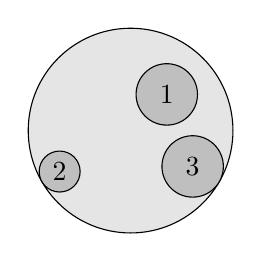
\begin{tikzpicture}[scale=1.3]
    \coordinate (a) at (45:0.5);
    \coordinate (b) at (210:0.8);
    \coordinate (c) at (-30:0.7);
    \filldraw [fill = gray!20] (0,0) circle (1);
    \filldraw [fill = gray!50] (a) circle (0.3) node {1};
    \filldraw [fill = gray!50] (b) circle (0.2) node {2};
    \filldraw [fill = gray!50] (c) circle (0.3) node {3};
  \end{tikzpicture}
\end{wrapfigure}


Un élément de $\DD_{n}(k)$ est une configuration ordonnée de $k$ petits $n$-disques aux intérieurs disjoints dans le disque unité $D^{n}$.
Chaque disque de la configuration s'obtient comme l'image d'un plongement de $D^{n}$ dans lui-même obtenu par la composition d'une translation et d'une homothétie.
L'ensemble $\DD_{n}(k)$ est muni de la topologie compacte-ouverte des plongements.
L'action du groupe symétrique réordonne les disques d'une configuration, et l'insertion est donnée par la composition des plongements.

\begin{center}
  \begin{tikzpicture}[scale=2]
  \coordinate (a) at (45:0.5);
  \coordinate (b) at (210:0.5);
  \coordinate (c) at (-30:0.8);
  \coordinate (d) at (80:0.5);
  \coordinate (e) at (0:0.7);

  \filldraw [fill = gray!20] (0,0) circle (1);
  \filldraw [fill = gray!50] (a) circle (0.4) node {1};
  \filldraw [fill = gray!50] (b) circle (0.5) node {2};
  \filldraw [fill = gray!50] (c) circle (0.2) node {3};

  \draw (1.3, 0) node {$\circ_{2}$};

  \coordinate (x1) at (2.5,0);
  \filldraw [fill = gray!20] (x1) circle (1);
  \filldraw [fill = gray!60!blue] ($(d) + (x1)$) circle (0.4) node {1};
  \filldraw [fill = gray!60!blue] ($(e) + (x1)$) circle (0.2) node {2};

  \draw (3.75, 0) node {$=$};

  \coordinate (x2) at (5,0);
  \filldraw [fill = gray!20] (x2) circle (1);
  \filldraw [fill = gray!50] ($(a) + (x2)$) circle (0.4) node {1};
  \draw [dashed] ($(b) + (x2)$) circle (0.5);
  \filldraw [fill = gray!50] ($(c) + (x2)$) circle (0.2) node {4};

  \coordinate (x3) at ($(x2) + (-0.433, -0.25)$); % cos(210)/2, sin(210)/2
  \filldraw [fill = gray!60!blue] ($1/2*(d) + (x3)$) circle (0.2) node {2};
  \filldraw [fill = gray!60!blue] ($1/2*(e) + (x3)$) circle (0.1) node {3};
\end{tikzpicture}

\end{center}

Un espace de lacets itéré $\Omega^{n} X$ est, presque par définition, une algèbre sur $\DD_{n}$.
Le «principe de reconnaissance»~\cite{May1972,BoardmanVogt1973} dit que la réciproque est vraie : sous des hypothèses techniques, une $\DD_{n}$-algèbre «group-like» est faiblement équivalente à un espace de $n$-lacets.

Les opérades des petits disques se sont révélées, depuis cette première application, être utiles dans de nombreux contextes.
Mentionnons la conjecture de Deligne~\cite{KontsevichSoibelman2000,McClureSmith2002}, qui dit que les cochaînes de Hochschild $C^{*}(A;A)$ d'une algèbre associative sont munies d'une action de $\DD_{2}$; le théorème de formalité des cochaînes de Hochschild et ses applications à la quantification des variétés de Poisson~\cite{Kontsevich1999,Tamarkin1998,Kontsevich2003}; le calcul de Goodwillie--Weiss et le calcul des espaces de plongements et des espaces de longs nœuds~\cite{Sinha2006,LambrechtsTurchinVolic2010,AroneTurchin2014,DwyerHess2012,BoavidaWeiss2013}, ainsi que l'homologie de factorisation, en quelque sorte la «version covariante» du calcul des plongements~\cite{BeilinsonDrinfeld2004,Lurie2009,Lurie2016,AyalaFrancis2015,CostelloGwilliam2017}.

Un résultat fondamental au sujet des opérades des petits disques est qu'elles sont \emph{formelles} sur $\Q$~\cite{Kontsevich1999,Tamarkin2003,LambrechtsVolic2014,FresseWillwacher2015}, c.-à-d. que l'opérade des chaînes $C_{*}(\DD_{n}; \Q)$ est quasi-isomorphe à son homologie $\en \coloneqq H_{*}(\DD_{n}; \Q)$.
Il suffit donc, sur $\Q$, d'étudier les opérades $\en$, qui ont une description combinatoire simple : $\en[1] = \Ass$ gouverne les algèbres associatives, et pour $n \geq 2$, $\en$ gouverne les $(n-1)$-algèbres de Poisson~\cite{Cohen1976}.
Quand $n = 2$, la formalité de l'opérade $\DD_{2}$ dépend du choix d'un associateur de Drinfeld, un objet qui définit une manière universelle de construire une catégorie monoïdale tressée à partir de données qui viennent de la théorie de Lie (voir p.ex.~\cite[Chapter~I.10]{Fresse2017} pour plus de détails).

\subsection*{Opérades «Swiss-Cheese»}

Les opérades colorées (aussi connues sous le nom de multicatégories) généralisent les opérades et sont utilisées pour décrire des structures algébriques à plusieurs objets.
Dans ce contexte, les entrées et la sortie d'une opération sont toutes étiquetées par une «couleur», et l'insertion n'est définie que si les couleurs correspondent.
Dans la définition d'une algèbre sur une opérade colorée, chaque couleur correspond à un objet donné.

\begin{wrapfigure}{l}{0.3\textwidth}
  \centering
  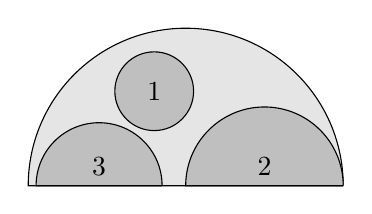
\begin{tikzpicture}
    \filldraw [fill = gray!20] (2,0) arc (0:180:2) -- (2,0);
    \filldraw [fill = gray!50] (2,0) arc (0:180:1) -- node[above] {$2$} (2,0);
    \filldraw [fill = gray!50] (-0.3,0) arc (0:180:0.8) -- node[above] {$3$} (-0.3,0);
    \filldraw [fill = gray!50] (-0.4,1.2) circle (0.5) node {$1$};
  \end{tikzpicture}
\end{wrapfigure}


L'opérade «Swiss-Cheese» $\SC = \SC_{2}$~\cite{Voronov1999} est une opérade à deux couleurs qui gouverne l'action d'une algèbre $\DD_{2}$ sur une algèbre $\DD_{1}$ par un morphisme central.
Une opération de $\SC$ est donné par le plongement de disques et de demi-disques dans le demi-disque unité supérieur.
Ces opérades sont liées aux OCHA de Kajiura et Stasheff~\cite{KajiuraStasheff2006a,Hoefel2009}, et il existe une version Swiss-Cheese de la conjecture de Deligne~\cite{DolgushevTamarkinTsygan2011}.
Des variantes en dimension supérieur $\SC_{n}$ gouvernent l'action d'une algèbre $\DD_{n}$ sur une algèbre $\DD_{n-1}$.
Contrairement aux opérades des petits disques, les opérades Swiss-Cheese ne sont pas formelles~\cite{Livernet2015}.

\subsection*{Espaces de configuration}

Soit $M$ une variété. Son $k$ième espace de configuration est donné par:
\[ \Conf_{k}(M) \coloneqq \{ x \in M^{k} \mid \forall i \neq j, \; x_{i} \neq x_{j} \}. \]
Les espaces de configuration sont intimement liés aux opérades des petits disques.
Par exemple, l'application $\DD_{n}(k) \to \Conf_{k}(\R^{n})$ qui associe à une configuration de disques la configuration constituée des centres des disques est une équivalence d'homotopie.

Cette construction n'est évidemment pas un invariant d'homotopie pour les variétés ouvertes dès que $k \geq 2$.
Par exemple, pour $n \in \mathbb{N}$, $\Conf_{2}(\R^{n}) \simeq S^{n-1}$.
Même en se restreignant aux variétés compactes sans bord, $\Conf_{k}(-)$ n'est pas un invariant d'homotopie~\cite{LongoniSalvatore2005}.
Le contre-exemple (donné par des espaces lenticulaires) n'est pas simplement connexe, et la question de savoir si $\Conf_{k}(-)$ est un invariant d'homotopie pour les variétés compactes, sans bord et simplement connexes reste ouverte.

Quelques résultats sont connus.
Le type d'homotopie de $\Omega \Conf_{k}(M)$ ne dépend que de celui de $(M, \partial M)$ pour les variétés compactes connexes~\cite{Levitt1995}.
Les espaces de configuration sont des invariants \emph{stables} d'homotopie des variétés compactes sans bord~\cite{AouinaKlein2004}.
Si $M$ est une variété projective lisse, alors le type d'homotopie rationnel de $\Conf_{k}(M)$ ne dépend que de celui de $M$.
Le même résultat est valable avec $k = 2$ pour les variétés compactes sans bord qui sont soit $2$-connexes~\cite{LambrechtsStanley2004}, soit simplement connexes et de dimension paire~\cite{CordovaBulens2015}.

\addsec{Résultats du Chapitre~\ref{chap.1}}

Comme mentionné précédemment, l'opérade Swiss-Cheese $\SC = \SC_{2}$ n'est pas formelle.
En d'autres termes, il n'est pas possible de récupérer le type d'homotopie de $\SC$ à partir de son homologie $\Sc = H_{*}(\SC)$.
Le but du premier chapitre de cette thèse est de trouver un modèle de $\SC$ qui corrige ce défaut de formalité.

Les trois opérades $\DD_{1}$, $\DD_{2}$ et $\SC$ sont asphériques, c.-à-d. que l'homotopie de chacun des espaces qui les composent est concentrée en degrés $0$ et $1$.
Il y a donc, pour chacune de ces opérades (notons les $\PP$), une équivalence d'homotopie canonique $\PP \qiso B \pi \PP$, où $B$ est le foncteur «espace classifiant» et $\pi$ le foncteur «groupoïde fondamental» (les deux étant fortement monoïdaux, ils préservent la structure d'opérade).
À homotopie près, il suffit donc d'étudier le groupoïde fondamental $\pi \PP$ de chacune de ces trois opérades $\PP \in \{ \DD_{1}, \DD_{2}, \SC \}$ à «équivalence catégorique» (morphisme d'opérade induisant une équivalence de catégorie en chaque arité) près.

Il existe des descriptions classiques de modèles en groupoïdes des deux opérades $\DD_{1}$ et $\DD_{2}$.
\begin{itemize}
\item En chaque arité, $\DD_{1}(r)$ est discret à homotopie près (avec $r!$ composantes connexes), et il est facile de voir que l'opérade
  $\pi \DD_{1}$ est faiblement équivalente à l'opérade $\PaP$ des permutations parenthésées.
  La catégorie $\PaP(r) = \Sigma_{r}$ est discrète, avec comme objets les permutations de $\{1,\dots,r\}$, et la structure d'opérade est donnée par la composition par blocs des permutations.
\item Les composantes $\DD_{2}(r)$ de l'opérade $\DD_{2}$ sont des espaces classifiants des groupes de tresses pures $P_{r}$.
  L'opérade $\pi \DD_{2}$ est ainsi faiblement équivalente à l'opérade $\PaB$ des tresses parenthésées (cf.~\cite[Chapter~I.3]{Fresse2017}, voir aussi~\cite{Fiedorowicz}).
  Les objets de $\PaB(r)$ sont encore les permutations de $\{1,\dots,r\}$.
  Les morphismes entre deux permutations $\sigma, \sigma' \in \PaB(r)$ sont les tresses colorées à $r$ brins entre ces deux permutations : chacun des brins de la tresse est «coloré» par un des nombres $\{1,\dots,r\}$, et l'ordre des brins au début (resp. à la fin) de la tresse est donné par $\sigma$ (resp. $\sigma'$).
  La composition des tresses est donnée par l'insertion d'une tresse dans un voisinage tubulaire d'un brin.
\end{itemize}

Le premier résultat de ce premier chapitre (Theorem~\ref{sw.thm.A}) est la définition d'une opérade en groupoïdes $\PaPB$ des tresses et permutations parenthésées.
Cette opérade combine, en quelque sorte, les deux opérades $\PaP$ et $\PaB$ pour obtenir une opérade colorée, et est faiblement équivalente au groupoïde fondamental $\pi \SC$.

La définition de $\PaPB$ est motivée par le résultat suivant.
L'homologie de l'opérade Swiss-Cheese se scinde en un «produit de Voronov» $\Sc = \en[2] \otimes \en[1]$, où $\en[1] = H_{*}(\DD_{1}) = \Ass$ gouverne les algèbres associatives et $\en[2] = H_{*}(\DD_{2}) = \Ger$ gouverne les algèbres de Gerstenhaber~\cite{Voronov1999}.
Concrètement, cela signifie qu'une algèbre sur $\Sc$ est la donnée d'un triplet $(A,B,f)$ où $A$ est une algèbre associative, $B$ est une algèbre de Gerstenhaber, et $f : B \to Z(A)$ est un morphisme d'algèbres de $B$ dans le centre de $A$.

Les algèbres (dans la catégorie des catégories) sur l'opérade $\PaP \simeq \pi \DD_{1}$ sont les catégories monoïdales, et les algèbres sur $\PaB \simeq \pi \DD_{2}$ sont les catégories monoïdales tressées.
En analogie avec le théorème de Voronov, nous démontrons que les algèbres (toujours dans la catégorie des catégories) sur $\PaPB \simeq \pi \SC$ sont les triplets $(\cM, \cN, F)$ où $\cM$ est une catégorie monoïdale, $\cN$ est une catégorie monoïdale tressée, et $F : \cM \to \Zd(\cN)$ est un foncteur monoïdal tressé de $\cM$ dans le centre de Drinfeld de $\cN$ -- un analogue catégorique du centre d'une algèbre associative.
Ce résultat est la contrepartie pour les opérades en groupoïdes de résultats $\infty$-catégoriques sur les algèbres à factorisation du demi-plan supérieur (cf.~\cite[Proposition 31]{Ginot2015} et~\cite[Example 2.13]{AyalaFrancisTanaka2017})

Dans une deuxième étape, nous fixons un associateur de Drindeld, que nous pouvons voir comme une équivalence rationnelle (au sens de la théorie de l'homotopie rationnelle) $\PaB_{+} \to \CDh_{+}$ où $\CDh_{+} = \operatorname{B} \hat{\mathbb{U}} \hat{\mathfrak{p}}_{+}$ est l'opérade complétée des diagrammes de cordes.
À partir de cette donnée, nous construisons une opérade $\PaPCD^{\varphi}$ rationnellement équivalente  à la complétion de l'opérade Swiss-Cheese.
Cette opérade étend la construction utilisée par Tamarkin~\cite{Tamarkin2003} pour démontrer la formalité de l'opérade $\DD_{2}$ et peut s'interpréter informellement comme un produit de Voronov tordu d'un modèle pour $\DD_{2}$ et d'un modèle pour $\DD_{1}$.

\addsec{Résultats du Chapitre~\ref{chap.2}}

Dans le second chapitre, nous étudions les espaces de configuration des variétés compactes sans bord simplement connexes.
Dans la suite, on note $M$ une telle variété.
Nous nous plaçons dans le cadre de la théorie de l'homotopie rationnelle de Sullivan, où les espaces sont modélisés par des algèbres différentielles graduées commutatives (CDGA en anglais) et nous cherchons à obtenir un modèle de $\Conf_{k}(M)$ pour $k \geq 0$.

La cohomologie d'une variété orientée compacte sans bord satisfait la dualité de Poincaré,  il y a un accouplement non dégénéré $H^{k}(M) \otimes H^{n-k}(M) \to \Q$ donné par $\alpha \otimes \beta \mapsto \alpha\beta \frown [M]$.
Lambrechts et Stanley~\cite{LambrechtsStanley2008} démontrent que si la variété est simplement connexe, alors cette propriété peut se traduire sur les modèles : $M$ admet un modèle rationnel $A$ à «dualité de Poincaré», c.-à-d. il y a un accouplement non-dégénéré $A^{k} \otimes A^{n - k} \to \Q$ induit par une «augmentation» $\varepsilon_{A} : A^{n} \rightarrow \Q$.
À partir d'un tel modèle à dualité de Poincaré, ils introduisent une CDGA $\GG{A}(k)$ et démontrent que les nombres de Betti rationnels de $\GG{A}(k)$ coïncident avec ceux de $\Conf_{k}(M)$~\cite{LambrechtsStanley2008a}.
Ils conjecturent que cette CDGA est en fait un modèle rationnel de $\Conf_{k}(M)$, ce qui est connu pour les variétés projectives lisses complexes~\cite{Kriz1994}, ainsi que quand $k = 2$ et que $M$ est $2$-connexe~\cite{LambrechtsStanley2004} ou de dimension paire~\cite{CordovaBulens2015}.

Cette CDGA avait déjà été étudiée dans certains cas particuliers~\cite{CohenTaylor1978,BenderskyGitler1991,Kriz1994,Totaro1996,FelixThomas2004}.
Elle admet une description simple pour les premières valeurs de $k$ : $\GG{A}(0) = \Q$ et $\GG{A}(1) = A$, ce qui est cohérent avec le fait que $\Conf_{0}(M) = \{*\}$ et $\Conf_{1}(M) = M$, et $\GG{A}(2)$ est quasi-isomorphe au quotient de $A^{\otimes 2}$ par l'idéal engendré par la «classe diagonale» de $A$ (le dual de Poincaré de $M \subset M \times M$).
Plus généralement, $\GG{A}(k)$ est en quelque sorte une version «étiquetée par $A$» de la description classique de la cohomologie de $\Conf_{k}(\R^{n})$~\cite{Arnold1969,Cohen1976}.

La formalité de l'opérade des petits disques entraîne en particulier que les espaces de configuration $\Conf_{k}(\R^{n})$ sont formels : la CDGA $H^{*}(\Conf_{k}(\R^{n})) \eqqcolon \enV(k)$ (avec la différentielle nulle) est un modèle rationnel de $\Conf_{k}(\R^{n})$.
La preuve par Kontsevich de cette formalité fournit des morphismes explicites~\cite{Kontsevich1999,LambrechtsVolic2014}.
L'idée de ce chapitre est d'adapter cette preuve aux espaces de configuration de $M$ pour obtenir le fait que $\GG{A}(k)$ est un modèle.

Cette preuve fait intervenir la compactification de Fulton--MacPherson des espaces de configuration~\cite{FultonMacPherson1994,AxelrodSinger1994}.
Étant donnée une variété $M$, l'espace $\FM_{M}(k)$ est une variété stratifiée dont l'intérieur est $\Conf_{k}(M)$.
Le bord de $\FM_{M}(k)$ est obtenu en autorisant les points d'une configuration à devenir infinitésimalement proches les uns des autres.
Il est possible de compactifier $\Conf_{k}(\R^{n})$ de manière similaire en un espace $\FM_{n}(k)$, en tenant compte du fait que $\R^{n}$ lui-même n'est pas compact.

La preuve passe par la définition d'un certain complexe de graphes intermédiaires $\Graphs_{n}(k)$.
On peut voir $H^{*}(\Conf_{k}(\R^{n})) = H^{*}(\FM_{n}(k))$ comme un quotient de $\Graphs_{n}(k)$ par un idéal acyclique.
Dans l'autre direction, il est nécessaire d'introduire le complexe des formes semi-algébriques par morceaux $\OmPA^{*}(\FM_{n}(k))$, qui est un modèle sur $\R$ de $\FM_{n}(k)$.
Un quasi-isomorphisme de $\Graphs_{n}(k)$ dans $\OmPA^{*}(\FM_{n}(k))$ est alors donné par des intégrales le long des fibres des projections canoniques $\FM_{n}(k+l) \rightarrow \FM_{n}(k)$.
Nous adaptons toutes ces constructions à $\Conf_{k}(M)$ pour obtenir un zigzag explicite de quasi-isomorphismes, pour $M$ une variété lisse compacte sans bord simplement connexe de dimension au moins $4$ :
\[ \GG{A}(k) \qiso* \Graphs_{R}(k) \qiso \OmPA^{*}(\FM_{M}(k)), \]
ce qui démontre que $\GG{A}(k)$ est un modèle sur $\R$ de $\FM_{M}(k) \simeq \Conf_{k}(\R^{n})$ (première partie du Theorem~\ref{cnf.thm.A}).
Le point clé de la preuve consiste à démontrer que pour les variétés simplement connexes de dimension $\geq 4$, la fonction de partition $\Zphi$, définie à l'aide d'intégrales sur $\FM_{M}$, est (presque) triviale, ce qui s'obtient à l'aide d'un argument de comptage de degré.

Si $A$ et $A'$ sont deux modèles de $M$, nous démontrons directement que $\GG{A}(k) \simeq_{\R} \GG{A'}(k)$, d'où l'invariance homotopique réelle de $\Conf_{k}(M)$ par rapport à $M$ (Corollary~\ref{cnf.cor.only-depends}).

On peut insérer une configuration de $\FM_{n}$ dans une autre, ce qui donne une structure d'opérade faiblement équivalent à l'opérade des petits disques $\DD_{n}$.
De même, quand $M$ est parallélisée, on peut insérer une configuration de $\FM_{n}$ dans une configuration de $\FM_{M}$ et obtenir ainsi une structure de $\FM_{n}$-module à droite sur $\FM_{M}$.
Quand $\chi(M) = 0$ (en particulier quand $M$ est parallélisée), il est facile d'observer que la collection $\GG{A} = \{ \GG{A}(k) \}$ est dotée d'une structure de comodule de Hopf à droite sur $H^{*}(\FM_{n}) = \enV$.
Nous démontrons que le zigzag de quasi-isomorphismes que nous construisons est compatible avec la structure de comodule quand $M$ est parallélisée (deuxième partie du Theorem~\ref{cnf.thm.A}).
En d'autres termes, nous obtenons un modèle réel du $\FM_{n}$-module à droite $\FM_{M}$.

Cela nous permet de calculer l'homologie de factorisation, un invariant des variétés.
Étant données une $n$-variété parallélisée $M$ et une $\FM_{n}$-algèbre $B$, l'homologie de factorisation de $M$ à coefficients dans $B$ peut se calculer comme le produit de composition relatif dérivé (cf.~\cite{AyalaFrancis2015} et~\cite[Section 5.1]{Turchin2013}) :
\[ \int_{M} B \coloneqq \FM_{M} \circ_{\FM_{n}}^{\mathbb{L}} B. \]
Notre résultat implique que si $M$ est une variété lisse compacte sans bord simplement connexe de dimension au moins $4$ et que $B$ est une $\en$-algèbre, alors l'homologie de factorisation de $M$ à coefficients dans $B$ est donnée, sur $\R$, par un complexe explicite :
\[ \int_{M} B \simeq \GG{A}^{\vee} \circ_{\en}^{\mathbb{L}} B. \]
Dans le cas où $B = S(\Sigma^{1-n} \mathfrak{g})$ est l'algèbre enveloppante supérieure d'une algèbre de Lie, nous reprenons des arguments de Félix et Thomas~\cite{FelixThomas2004} pour démontrer que $\int_{M} S(\Sigma^{1-n} \mathfrak{g})$ se calcule avec un complexe de Chevalley--Eilenberg (Proposition~\ref{cnf.prop.cmp-knudsen}), un résultat précédemment obtenu par Knudsen~\cite{Knudsen2016} par des méthodes complètement différentes.

Enfin, en utilisant la preuve de Giansiracusa et Salvatore~\cite{GiansiracusaSalvatore2010} de la formalité de l'opérade des petits disques à repère, nous généralisons notre résultat à $S^{2}$, la seule surface simplement connexe (Theorem~\ref{cnf.thm.framed}).

\addsec{Résultats du Chapitre~\ref{chap.3}}

Dans le troisième chapitre, nous étendons les résultats précédents à une large classe de variétés à bord.

Nous nous concentrons sur le cas des variétés admettant un «modèle à dualité de Poincaré--Lefschetz».
Cette notion est une généralisation de «joli modèle surjectif» (\emph{``surjective pretty model''} en anglais), une notion due à Cordova Bulens, Lambrechts et Stanley~\cite{CordovaBulensLambrechtsStanley2015} (voir aussi~\cite{LambrechtsStanley2005}).
L'intuition derrière cette notion provient de la dualité de Poincaré--Lefschetz.
Soit $N$ une variété orientée compacte sans bord de dimension $n$ et $K \subset N$ un sous-polyhèdre, et soit $M = N - \tilde{K}$ est la variété à bord obtenue en retirant un épaississement de $K$.
Alors la cohomologie de $M$ se calcule à partir de la cohomologie de $N$ en «tuant» les classes duales des classes d'homologie provenant de $K$.
Concrètement, un joli modèle surjectif est construit à partir des données suivantes :
\begin{itemize}
\item une CDGA à dualité de Poincaré $P$ (correspondant à un modèle de $N$) ;
\item une CDGA connexe $Q$ satisfaisant $Q^{\geq n/2 -1} = 0$ (correspondant à un modèle de $K$) ;
\item un morphisme surjectif de CDGAS $\psi : P \to Q$.
\end{itemize}

La dualité de Poincaré de $P$ induit un isomorphisme $\theta_{P} : P \to P^{\vee}[-n]$ entre $P$ et la désuspension de son dual.
On définit l'application $\psi^{!} : Q^{\vee}[-n] \to P$ comme la composition $\theta^{-1}_{P} \circ \psi^{\vee}[-n]$.
Notons que $\psi\psi^{!} = 0$ pour des raisons de degré.
Le joli modèle surjectif (correspondant à un modèle de l'inclusion $\partial M \subset M = N - K$) associé à $\psi : P \to Q$ est alors donné par :
\[ \lambda = \psi \oplus \id : B = P \oplus_{\psi^{!}} Q^{\vee}[1-n] \to B_{\partial} = Q \oplus Q^{\vee}[1-n], \]
où $P \oplus_{\psi^{!}} Q^{\vee}[1-n]$ est le cône (conoyau homotopique) de $\psi^{!}$.
La CDGA $B_{\partial}$ est une CDGA à dualité de Poincaré de dimension formelle $n-1$, et $B$ est quasi-isomorphe au quotient $A = P/I$ de la CDGA à dualité de Poincaré $P$ par son idéal $I = \im \psi^{!}$.
La dualité de Poincaré--Lefschetz se traduit en l'existence d'un isomorphisme $A \cong K^{\vee}[-n]$, où $K = \ker \psi \cong \ker \lambda$ est un modèle des formes relatives sur $(M, \partial M)$.

Un exemple éclairant de joli modèle surjectif est celui de $(M, \partial M) = (D^{n}, S^{n-1})$.
On peut voir $M = D^{n}$ comme une sphère $N = S^{n}$ à laquelle on a retiré l'épaississement d'un point $K = \{*\}$.
En appliquant le dictionnaire ci-dessus, on prend donc $P = H^{*}(S^{n}) = S(\vol_{n})/(\vol_{n}^{2})$ comme modèle de $N$ et $Q = H^{*}(\{*\}) = \R$ comme modèle de $K$, l'application $\psi : P \to Q$ étant simplement l'augmentation.
L'application $\psi^{!} : Q^{\vee}[-n] \to P$ est donnée par $\psi^{!}(1_{Q}^{\vee}) = \vol_{n}$.
Le modèle $P \oplus_{\psi^{!}} Q^{\vee}[1-n]$ est de dimension $3$, engendré par $1_{P}$ en degré $0$, $1_{Q}^{\vee}$ en degré $n-1$ et $\vol_{n}$ en degré $n$.
Tous les produits non-triviaux sont nuls et $d(1_{Q}^{\vee}) = \vol_{n}$.

Nous ne savons pas si toutes les variétés orientées à bord admettent un joli modèle surjectif, contrairement aux variétés simplement connexes (donc orientées) sans bord qui admettent toutes un modèle à dualité de Poincaré.
Si $M$ et $\partial M$ sont simplement connexes, nous pouvons, sous l'hypothèse supplémentaire que $\dim M \geq 7$, construire ce que nous appelons un «modèle à dualité de Poincaré--Lefschetz» $\lambda : B \to B_{\partial}$ de $(M, \partial M)$.
La caractéristique principale de ces modèles est l'existence d'un accouplement non-dégénéré entre un quotient $A \coloneqq B/\ker \theta \simeq B$ et le noyau de $\lambda$ qui modélise l'accouplement entre $H^{*}(M)$ et $H^{*}(M, \partial M)$, comme pour les jolis modèles surjectifs.
L'existence d'un modèle à DPL est suffisante pour reprendre toutes les constructions précédentes et obtenir le même modèle $\GG{A}(k)$ de $\OmPA^{*}(\Conf_{k}(M))$, ainsi que le modèle $\SGraphs_{R}^{\varphi}$ de $\OmPA^{*}(\SFM_{M})$ (tout en étant compatible avec les structures de comodule si $M$ est parallélisée).

À partir d'un tel joli modèle surjectif, il est possible de reprendre presque mot pour mot la définition de $\GG{A}(k)$ du Chapitre~\ref{chap.2}.
Si par exemple $M = D^{n}$, nous obtenons $\GG{A} \cong \enV$ vu comme un comodule à droite sur lui-même.
En réutilisant les techniques du Chapitre~\ref{chap.2}, nous démontrons que $\GG{A}(k)$ a les mêmes nombres de Betti sur $\Q$ que $\Conf_{k}(M)$.
Nous définissons également une version «perturbée» $\GGt{A}$ de $\GG{A}$, qui est isomorphe à $\GG{A}$ comme dg-module mais pas comme algèbre, et nous montrons que $\GG{A}(k)$ est un modèle sur $\R$ de $\Conf_{k}(M)$.

Il est possible d'adapter la compactification de Fulton--MacPherson $\FM_{M}$ aux variétés compactes à bord, en autorisant des points à devenir infinitésimalement proches les uns des autres, mais aussi en autorisant des points de l'intérieur de la variété à devenir infinitésimalement proches du bord.
On obtient ainsi une compactification de l'espace de configuration coloré :
\begin{align*}
  \Conf_{k,l}(M)
  & \coloneqq \{ (x_{1}, \dots, x_{k}, y_{1}, \dots, y_{l}) \in \Conf_{k+l}(M) \mid x_{i} \in \partial M, y_{j} \in \mathring{M} \} \\
  & \xhookrightarrow{\sim} \SFM_{M}(k,l).
\end{align*}

Si $M$ est parallélisée, la collection $\SFM_{M} = \{ \SFM_{M}(k,l) \}_{k \geq 0, l \geq 0}$ est un module à droite sur une opérade $\SFM_{n}$ qui est construite de manière similaire à $\FM_{n}$ et est faiblement équivalent à l'opérade Swiss-Cheese $n$-dimensionnelle.

Willwacher~\cite{Willwacher2015a} a construit un modèle en graphes $\SGraphs_{n}$ de l'opérade $\SFM_{n}$, similaire au modèle $\Graphs_{n}$ de Kontsevich pour l'opérade $\FM_{n}$.
Comme dans le Chapitre~\ref{chap.2}, nous adaptons la construction de Willwacher au «cas étiqueté» pour construire un comodule de Hopf à droite $\SGraphs^{c_{\varphi},\szphi}_{R}$ sur $\SGraphs_{n}$, et nous obtenons des quasi-isomorphismes de CDGAs (compatibles avec les structures de comodule le cas échéant) :
\begin{align*}
  {} & \SGraphs^{\varphi}_{R}(k,l) \qiso \OmPA^{*}(\SFM_{M}(k,l)), \\
  \GG{A}(l) & \qiso* \SGraphs^{c_{\varphi},\szphi}_{R}(0,l) \qiso \OmPA^{*}(\SFM_{M}(0,l)) \simeq \OmPA^{*}(\Conf_{l}(M)).
\end{align*}
